
\let\negmedspace\undefined
\let\negthickspace\undefined
\documentclass[journal]{IEEEtran}
\usepackage[a5paper, margin=10mm, onecolumn]{geometry}
%\usepackage{lmodern} % Ensure lmodern is loaded for pdflatex
\usepackage{tfrupee} % Include tfrupee package
\setlength{\headheight}{1cm} % Set the height of the header box
\setlength{\headsep}{0mm}     % Set the distance between the header box and the top of the text
\usepackage{gvv-book}
\usepackage{gvv}
\usepackage{cite}
\usepackage{amsmath,amssymb,amsfonts,amsthm}
\usepackage{algorithmic}
\usepackage{graphicx}
\usepackage{textcomp}
\usepackage{xcolor}
\usepackage{txfonts}
\usepackage{listings}
\usepackage{enumitem}
\usepackage{mathtools}
\usepackage{gensymb}
\usepackage{comment}
\usepackage[breaklinks=true]{hyperref}
\usepackage{tkz-euclide} 
\usepackage{listings}
% \usepackage{gvv}                                        
\def\inputGnumericTable{}                                 
\usepackage[latin1]{inputenc}                                
\usepackage{color}                                            
\usepackage{array}                                            
\usepackage{longtable}                                       
\usepackage{calc}                                             
\usepackage{multirow}                                         
\usepackage{hhline}                                           
\usepackage{ifthen}                                           
\usepackage{lscape}
\renewcommand{\thefigure}{\theenumi}
\renewcommand{\thetable}{\theenumi}
\setlength{\intextsep}{10pt} % Space between text and floats
\numberwithin{equation}{enumi}
\numberwithin{figure}{enumi}
\renewcommand{\thetable}{\theenumi}
\begin{document}
\bibliographystyle{IEEEtran}
\title{11.16.3.7}
\author{EE24BTECH11041 - Mohit}
% \maketitle
% \newpage
% \bigskip
{\let\newpage\relax\maketitle}
\textbf{Question:-} A fair coin is tossed four times, and a person wins Rs.1 for each head and loses Rs.1.50 for each tail. From the sample space, calculate how many different amounts of money you can have after four tosses and the probability of having each of these amounts.

\textbf{Solution}

\subsection*{Step 1: Net Money Calculation}

Let:
\[
H = +1 \quad \text{(gain Rs.1 for Head)}, \quad T = -1.50 \quad \text{(lose Rs.1.50 for Tail)}.
\]

For \( x \), the number of heads in 4 tosses, the total net money can be calculated using the formula:
\[
\text{Net Money} = x(1) + (4-x)(-1.5)
\]
\[
\text{Net Money} = x - 1.5(4-x)
\]
\[
\text{Net Money} = 2.5x - 6,
\]
where \( x = 0, 1, 2, 3, 4 \).

\subsection*{Step 2: Possible Outcomes and Net Money}

\begin{itemize}
    \item \( x = 0 \): All tails (\( TTTT \)):
    \[
    \text{Net Money} = 2.5(0) - 6 = -6
    \]
    \item \( x = 1 \): One head, three tails (\( HTTT, THTT, TTHT, TTTH \), etc.):
    \[
    \text{Net Money} = 2.5(1) - 6 = -3.5
    \]
    \item \( x = 2 \): Two heads, two tails (\( HHTT, HTHT, HTTH, \dots \)):
    \[
    \text{Net Money} = 2.5(2) - 6 = -1
    \]
    \item \( x = 3 \): Three heads, one tail (\( HHHT, HHTH, HTHH, THHH \)):
    \[
    \text{Net Money} = 2.5(3) - 6 = 1.5
    \]
    \item \( x = 4 \): All heads (\( HHHH \)):
    \[
    \text{Net Money} = 2.5(4) - 6 = 4
    \]
\end{itemize}

\subsection*{Step 3: Number of Outcomes for Each Case}

The number of outcomes for each \( x \) is given by the binomial coefficient \( \binom{4}{x} \):
\[
\begin{aligned}
    &x = 0: \binom{4}{0} = 1, \\
    &x = 1: \binom{4}{1} = 4, \\
    &x = 2: \binom{4}{2} = 6, \\
    &x = 3: \binom{4}{3} = 4, \\
    &x = 4: \binom{4}{4} = 1.
\end{aligned}
\]

\subsection*{Step 4: Probabilities of Each Case}

Since the coin is fair, the probability of each outcome is \( \frac{1}{16} \). The probabilities for each \( x \) are:
\[
\begin{aligned}
    &x = 0: \text{Probability} = \frac{\binom{4}{0}}{16} = \frac{1}{16}, \\
    &x = 1: \text{Probability} = \frac{\binom{4}{1}}{16} = \frac{4}{16} = \frac{1}{4}, \\
    &x = 2: \text{Probability} = \frac{\binom{4}{2}}{16} = \frac{6}{16} = \frac{3}{8}, \\
    &x = 3: \text{Probability} = \frac{\binom{4}{3}}{16} = \frac{4}{16} = \frac{1}{4}, \\
    &x = 4: \text{Probability} = \frac{\binom{4}{4}}{16} = \frac{1}{16}.
\end{aligned}
\]

\subsection*{Step 5: Final Answer}

The different amounts of money and their probabilities are summarized below:

\[
\begin{array}{|c|c|}
\hline
\text{Net Money (Rs)} & \text{Probability} \\
\hline
-6 & \frac{1}{16} \\
-3.5 & \frac{1}{4} \\
-1 & \frac{3}{8} \\
1.5 & \frac{1}{4} \\
4 & \frac{1}{16} \\
\hline
\end{array}
\]
\textbf{CODING LOGIC:-}


\subsection*{1.C Code Description}

The C program computes the net money for a given sequence of coin tosses. The outcomes are represented as a string, where:
\begin{enumerate}
    \item Each \textbf{H} (head) contributes Rs.1 to the net money.
    \item Each \textbf{T} (tail) deducts Rs.1.50 from the net money.
\end{enumerate}
The program performs the following steps:
\begin{enumerate}
    \item Accepts a string of coin toss outcomes (e.g., \texttt{"HHTT"}).
    \item Iterates through the string, updating the net money:
    \begin{itemize}
        \item Add Rs.1 for each \texttt{H}.
        \item Subtract Rs.1.50 for each \texttt{T}.
    \end{itemize}
    \item Returns the final net money.
\end{enumerate}

\subsection*{2.Python Code Description}

The Python code performs the following:
\begin{enumerate}
    \item Simulates a specified number of random coin tosses (e.g., 100,000 trials).
    \item Calls the C function for each outcome to compute the net money.
    \item Counts the occurrences of each net money value and calculates their probabilities using:
    \[
    P(\text{Net Money} = x) = \frac{\text{Frequency of } x}{\text{Total Simulations}}
    \]
    \item Plots the probability distribution using \texttt{matplotlib}.
\end{enumerate}

\subsection*{3.Graphical Output}

The Python code generates a bar chart where:
\begin{itemize}
    \item The x-axis represents the possible net money values (\( -6, -3.5, -1, 1.5, 4 \)).
    \item The y-axis represents the probabilities, ranging from 0 to 1.
    \item Each bar corresponds to the probability of a specific net money value.
\end{itemize}

\subsection*{4.Probability Mass Function (PMF)}

The PMF represents the probability of each possible net money value. For 4 coin tosses, the possible net money values and their probabilities are:

\[
S = \{-6, -3.5, -1, 1.5, 4\}
\]

\[
P(\text{Net Money} = x) =
\begin{cases}
\frac{1}{16}, & x = -6 \\
\frac{1}{4}, & x = -3.5 \\
\frac{3}{8}, & x = -1 \\
\frac{1}{4}, & x = 1.5 \\
\frac{1}{16}, & x = 4 \\
0, & x \notin S
\end{cases}
\]

\subsection*{5.Cumulative Distribution Function (CDF)}

The CDF represents the cumulative probability of outcomes up to a given value \(x\), defined as:
\[
F(x) = P(\text{Net Money} \leq x) = \sum_{k \leq x} P(\text{Net Money} = k)
\]

For the coin toss:
\[
F(x) =
\begin{cases}
0, & x < -6 \\
\frac{1}{16}, & -6 \leq x < -3.5 \\
\frac{5}{16}, & -3.5 \leq x < -1 \\
\frac{7}{16}, & -1 \leq x < 1.5 \\
\frac{15}{16}, & 1.5 \leq x < 4 \\
1, & x \geq 4
\end{cases}
\]

\subsection*{6.Simulation Process}

The Python simulation performs the following steps:
\begin{enumerate}
    \item Simulates 4 coin tosses for each trial using random choices of \texttt{'H'} and \texttt{'T'}.
    \item Calls the C function to compute the net money for each simulated outcome.
    \item Tracks the frequency of each net money value over all trials.
    \item Calculates probabilities from the frequencies:
    \[
    P(x) = \frac{\text{Frequency of } x}{\text{Total Trials}}
    \]
    \item Plots the PMF and calculates the CDF.
\end{enumerate}

\begin{figure}[h!]
   \centering
   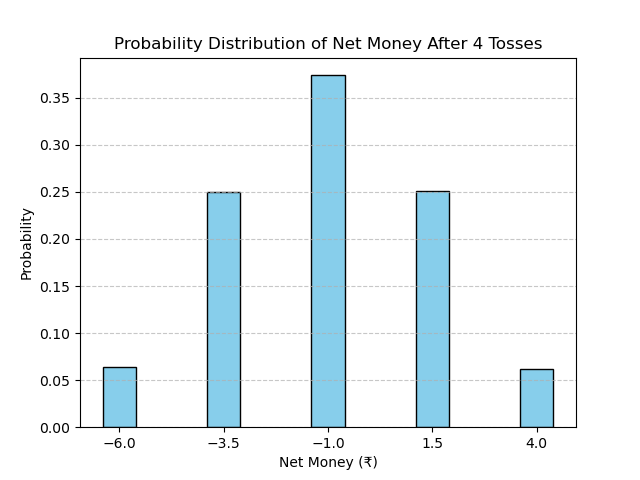
\includegraphics[width=0.7\linewidth]{figs/Figure_1.png}
\end{figure}

\end{document}
